\section{Korrelationsgrafer}
\label{DatabehandlingKorrelationsgrafer}
% SKRIV AT DER IKKE TAGES HØJDE FOR GRUPPER ELLER PCA'ER
%DER SKAL VÆRE BESVARELSER PÅ BEGGE SKALAER, ELLERS SLETTES PUNKTET
Som beskrevet udføres der en PCA analyse relativt til forskellige grupperinger. Ud fra disse PCA analyser forefindes der korrelation mellem nogen af de fundne og testede parametre. For yderliger at undersøge disse korrelationer opsættes relevante grafer, hvor forholdet mellem de forskellige parametre og skala spørgsmål visualiseres. På alle grafer i det følgende afsnit vil x-aksen indikere testpersoner, men ikke nødvendigvis i kronologisk rækkefølge, hvorfor værdier på x-aksen er fjernet.

\subsubsection{Korrelation relativt til højde}
Når PCA analysen udføres relativt til højde, tyder det, som beskrevet i \fullref{DatabehandlingRHeight}, på, at en positiv korrelation mellem følgende parametre finder sted:
\begin{itemize}
	\item SQ12 og SQ18
	\item SQ10 OG SQ13 (MANGLER FIGUR)
	\item SQ14 og SQ15
	\item SQ8 og SQ17\blankline
\end{itemize}
\noindent
%
Derudover forefindes der negativ korrelation mellem følgende parametre:
\begin{itemize}
	\item SQ12 og S21
	\item SQ18 og SQ21
	\item SQ2 og SQ9
	\item SQ4 og SQ9
	\item SQ16 og SQ19\blankline
\end{itemize}
\noindent
%
Korrelationen mellem SQ12 og SQ18 skyldes ikke at de måler det samme, men derimod at når testpersonerne godt kan lide at blive betjent af robotten, så synes de også robotten er spændende, hvilket fremgår på \autoref{fig:SammenligningSQ12SQ18}. 
%
\begin{figure}[H]
	\centering
	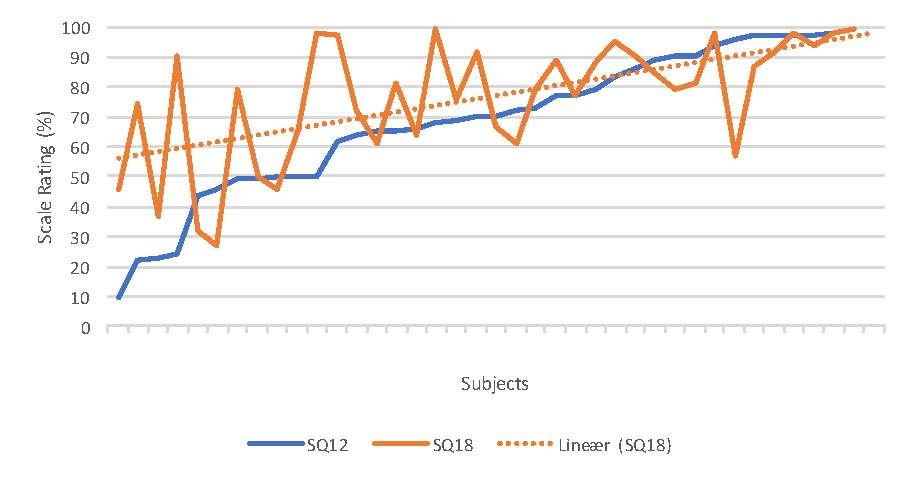
\includegraphics[width=\textwidth]{Figure/Korrelationsgrafer/SQ12+SQ18}
	\caption{Sammenhæng mellem hvad testpersonerne angiver (\%) på skalaen til SQ12: \textit{Jeg kan godt lide at blive betjent af robotten} og SQ18: \textit{Hvad synes du om robotten?}. At den orange kurve ikke er kontinuerlig skyldes, at nogle testpersoner ikke har angivet en respons på skalaen.}
	\label{fig:SammenligningSQ12SQ18}
\end{figure}
\noindent
%
Korrelationen mellem SQ14 og SQ15 skyldes ikke at de måler det samme, og ud fra tendenslinjen på \autoref{fig:SammenligningSQ14SQ15} tyder det på, at der tilnærmelsesvis er en sammenhæng mellem de to parametre. Fokuseres der derimod på punkterne på graferne virker det ikke som om, at der er en korrelation mellem hvor overrasket testpersonerne bliver og hvor personlig robottens hjælp opleves.
%
\begin{figure}[H]
	\centering
	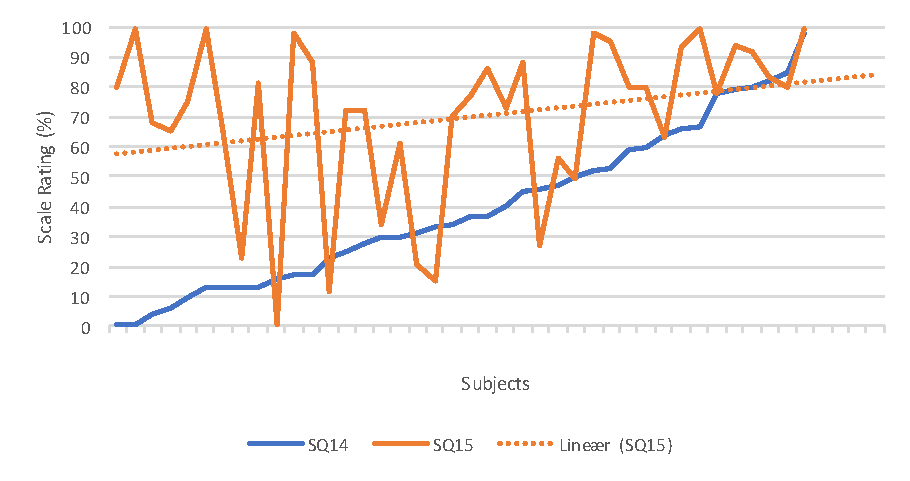
\includegraphics[width=\textwidth]{Figure/Korrelationsgrafer/SQ14+SQ15}
	\caption{Sammenhæng mellem hvad testpersonerne angiver (\%) på skalaen til SQ14: \textit{Hvor personlig oplevede du robottens hjælp?} og SQ15: \textit{Hvor overrasket blev du over robottens henvendelse?}.}
	\label{fig:SammenligningSQ14SQ15}
\end{figure}
\noindent
% SKRIV AT DET TYDER PÅ KORRELATION
Korrelationen mellem SQ8 og SQ17 skyldes ikke at de måler det sammen, det tyder derimod på, at korrelationen forekommer når testpersonerne føler, at robotten kan hjælpe dem og samtidig vurderer at robotten er elegant. Dog er denne korrelation lille, fordi datapunkterne varierer en del, særligt i forhold til SQ17, jævnfør \autoref{fig:SammenligningSQ8SQ17}.  
%
\begin{figure}[H]
	\centering
	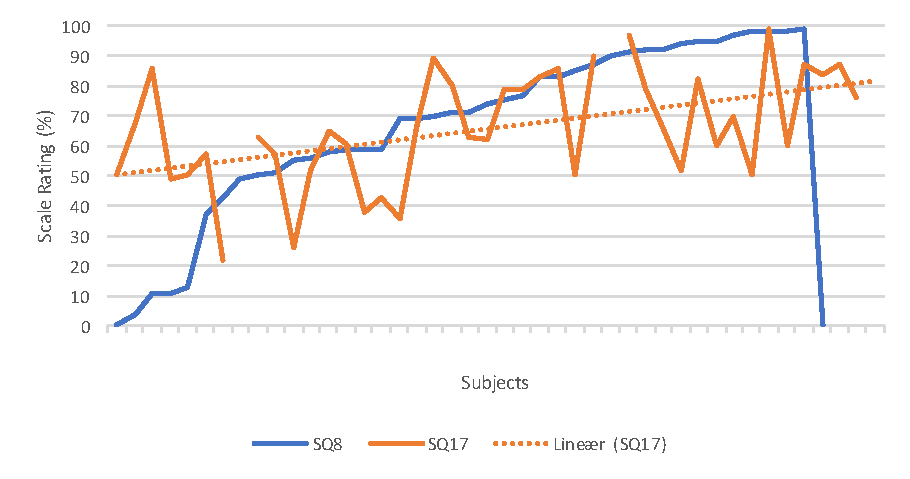
\includegraphics[width=\textwidth]{Figure/Korrelationsgrafer/SQ8+SQ17}
	\caption{Sammenhæng mellem hvad testpersonerne angiver (\%) på skalaen til SQ8: \textit{Jeg føler, at robotten kan hjælpe mig} og SQ17: \textit{Hvad synes du om robotten?}. At den orange kurve ikke er kontinuerlig skyldes, at nogle testpersoner ikke har angivet en respons på skalaen.}
	\label{fig:SammenligningSQ8SQ17}
\end{figure}
\noindent
I forhold til den negative korrelation mellem SQ21 og SQ12, vedrørende hvor godt testpersonerne kan lide at blive betjent af robotten, fremgår det ud fra \autoref{fig:SammenligningSQ12SQ21}, at når at desto mindre anmassende robotten opleves, desto bedre kan testpersonerne lide at blive betjent af robotten, hvilket giver god mening. 
%
\begin{figure}[H]
	\centering
	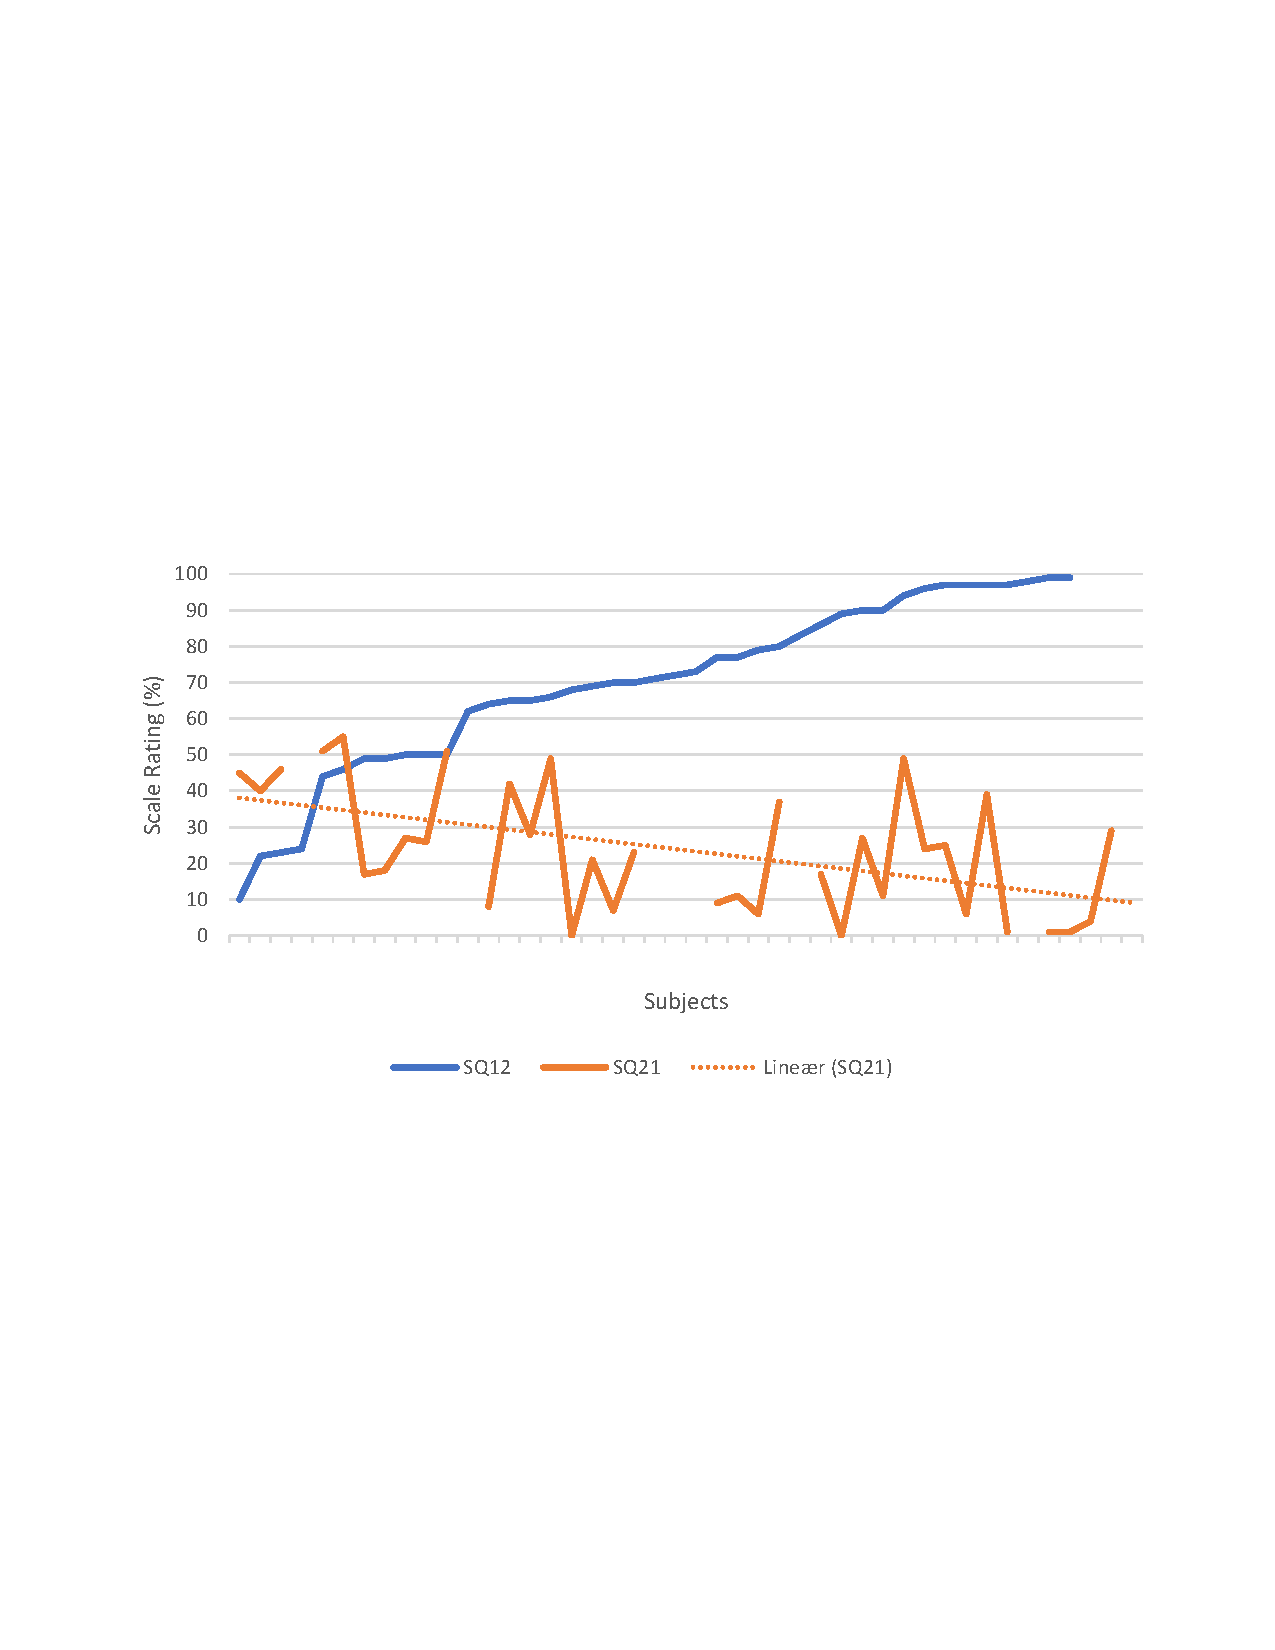
\includegraphics[width=\textwidth]{Figure/Korrelationsgrafer/SQ12+SQ21}
	\caption{Sammenhæng mellem hvad testpersonerne angiver (\%) på skalaen til SQ12: \textit{Jeg kan godt lide at blive betjent af robotten} og SQ21: \textit{Hvad synes du ellers om robotten?}. At den orange kurve ikke er kontinuerlig skyldes, at nogle testpersoner ikke har angivet en respons på skalaen.}
	\label{fig:SammenligningSQ12SQ21}
\end{figure}
\noindent
%
I forohold til den negative korrelation mellem SQ18, vedrørende hvor spændende robotten opleves, og SQ21, fremgår det at ud fra \autoref{fig:SammenligningSQ18SQ21}, at desto mindre anmassende robotten opleves desto mere spændende vurderes robotten. DOG TYDER DET PÅ AT NÅR SQ18 ER HØJEST SÅ STIGER SQ21
%
\begin{figure}[H]
	\centering
	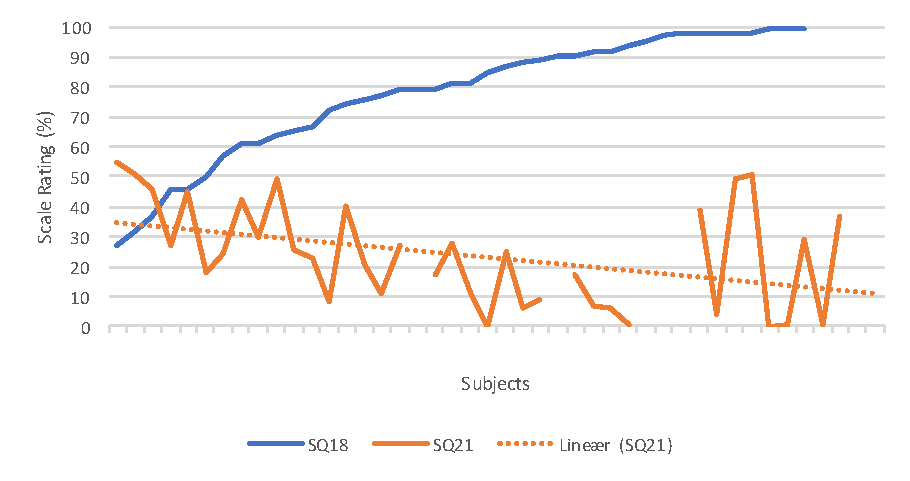
\includegraphics[width=\textwidth]{Figure/Korrelationsgrafer/SQ18+SQ21}
	\caption{Sammenhæng mellem hvad testpersonerne angiver (\%) på skalaen til SQ18: \textit{Hvad synes du om robotten?}, i forhold til \textit{spændende}, og SQ21: \textit{Hvad synes du ellers om robotten?}, i forhold til \textit{anmassende}. At den orange kurve ikke er kontinuerlig skyldes, at nogle testpersoner ikke har angivet en respons på skalaen.}
	\label{fig:SammenligningSQ18SQ21}
\end{figure}
\noindent
%
I henhold til den negative korrelation mellem SQ2, vedrørende hvorvidt robotten er imødekommende eller afvisende, og SQ9, fremgår det at desto mere imødekommende robotten opleves, desto mindre er den i vejen, jævnfør \autoref{fig:SammenligningSQ2SQ9}.
%
\begin{figure}[H]
	\centering
	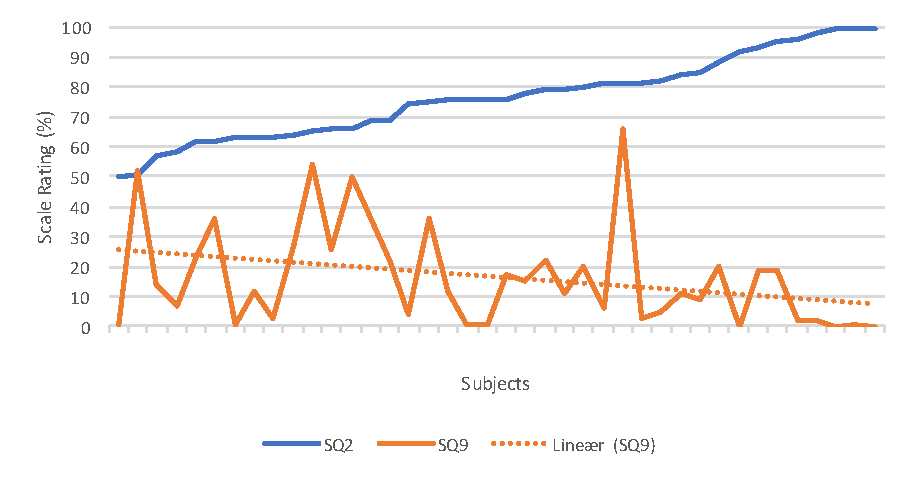
\includegraphics[width=\textwidth]{Figure/Korrelationsgrafer/SQ2+SQ9}
	\caption{Sammenhæng mellem hvad testpersonerne angiver (\%) på skalaen til SQ2: \textit{Hvordan oplevede du robotten?}, i forhold til \textit{afvisende} og \textit{imødekommende}, og SQ9: \textit{Jeg synes, at robotten stod i vejen}. At den orange kurve ikke er kontinuerlig skyldes, at nogle testpersoner ikke har angivet en respons på skalaen.}
	\label{fig:SammenligningSQ2SQ9}
\end{figure}
\noindent
%
Selvom det på \autoref{fig:RHeight-Biplot} tyder på, at der er en negativ korrelation mellem SQ4, vedrørende robottens bevægelser, og SQ9, så fremgår denne korrelation ikke som negativ på \autoref{fig:RHeight-3D} eller på \autoref{fig:SammenligningSQ4SQ9}, at dette ikke nødvendigvis er tilfældet.
%
\begin{figure}[H]
	\centering
	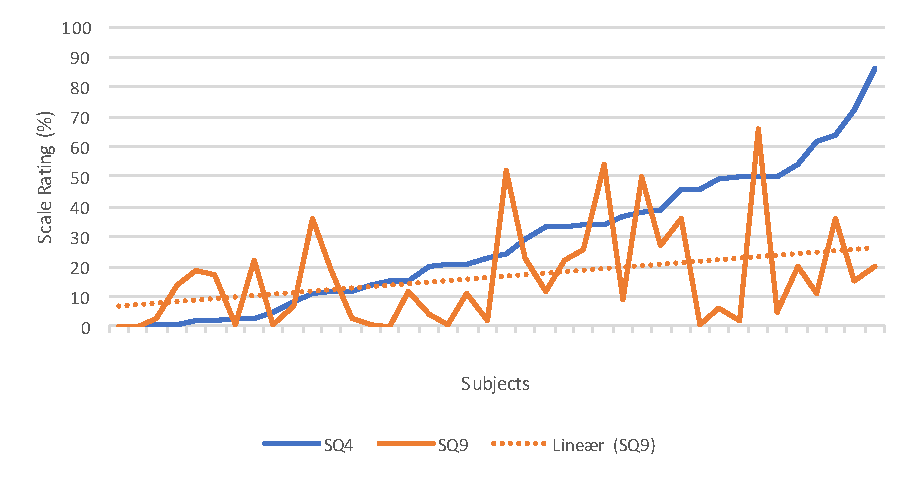
\includegraphics[width=\textwidth]{Figure/Korrelationsgrafer/SQ4+SQ9}
	\caption{Sammenhæng mellem hvad testpersonerne angiver (\%) på skalaen til SQ4: \textit{Hvordan oplevede du robottens bevægelser?}, i forhold til \textit{vilde} og \textit{rolige} og SQ9: \textit{Jeg synes, at robotten stod i vejen}. At den orange kurve ikke er kontinuerlig skyldes, at nogle testpersoner ikke har angivet en respons på skalaen.}
	\label{fig:SammenligningSQ4SQ9}
\end{figure}
\noindent
%
Den negative korrelation mellem SQ16 og SQ19 forekommer både på \autoref{fig:RHeight-Biplot} og på \autoref{fig:RHeight-3D}, men korrelationen er ikke lige så markant på \autoref{fig:SammenligningSQ16SQ19}, da datapunkterne for SQ19 varierer en del.  
%
\begin{figure}[H]
	\centering
	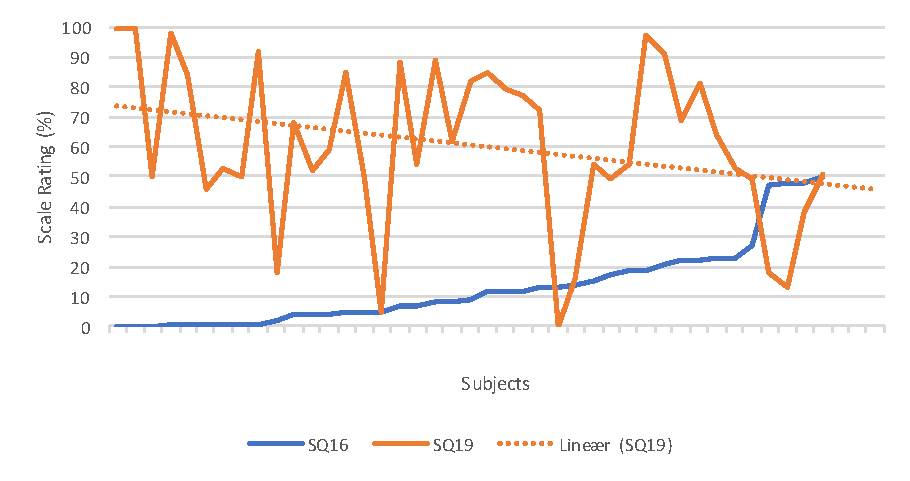
\includegraphics[width=\textwidth]{Figure/Korrelationsgrafer/SQ16+SQ19}
	\caption{Sammenhæng mellem hvad testpersonerne angiver (\%) på skalaen til SQ16 og SQ19, der begge har samme skala spørgsmål: \textit{Hvad synes du om robotten?}, men vedrører henholdvist \textit{irriterende} og \textit{sød}.}
	\label{fig:SammenligningSQ16SQ19}
\end{figure}
\noindent
%








\subsubsection{Korrelation relativt til afstand}
Når PCA analysen udføres relativt til afstand, tyder det, som beskrevet i \fullref{DatabehandlingRAfstand}, på, at en positiv korrelation mellem følgende parametre finder sted:
\begin{itemize}
	\item SQ1 og SQ12
	\item SQ7 og SQ17
	\item SQ10 og SQ22
	\item SQ8 og SQ21
\end{itemize}
%
Derudover ses der negativ korrelation mellem følgende parametre:
\begin{itemize}
	\item SQ2 og SQ9
	\item SQ14 og SQ16
	\item SQ10 og SQ13
	\item SQ13 og SQ22
	\item SQ5 og SQ8
	\item SQ5 og SQ21
	\item SQ19 og SQ20
\end{itemize}

Laves graferne for sammenhængen for SQ1 og SQ12 samt SQ7 og SQ17 ses der ikke nogen relevant sammenhæng, hvorfor disse kun er at finde i det elektroniske bilag, \fullref{ELEKTRONISK BILAG}.

På \autoref{fig:SammenligningSQ10SQ22} ses sammenhængen mellem SQ10 og SQ22. Det ses at deE IKKE tendens af, at testpersonerne synes robotten er mere sjov, når de samtidig føler sig mere tryg ved robotten. INGEN KORRELATION
%
\begin{figure}[H]
	\centering
	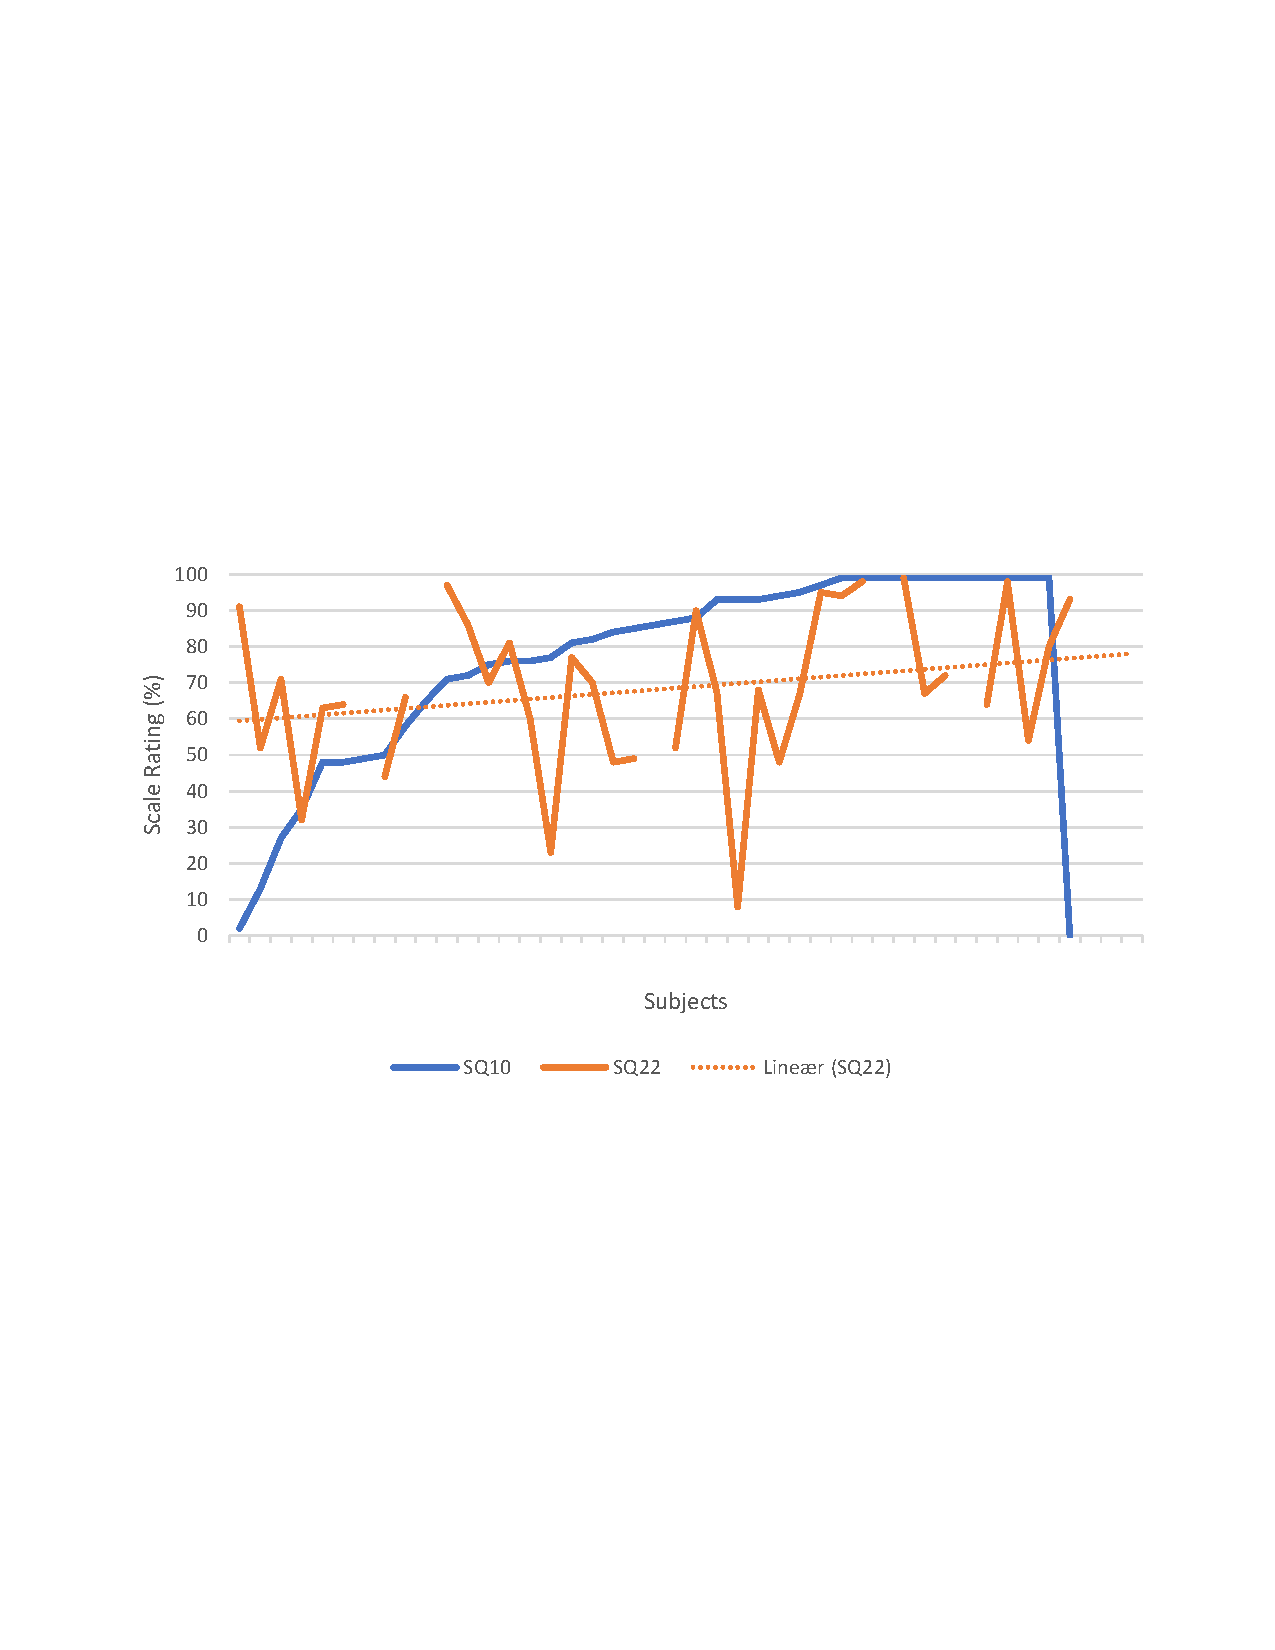
\includegraphics[width=\textwidth]{Figure/Korrelationsgrafer/SQ10+SQ22}
	\caption{Sammenhæng mellem hvad testpersonerne angiver (\%) på skalaen til SQ10: \textit{Jeg føler mig tryg ved robotten} og SQ22: \textit{Hvad synes du ellers om robotten?}. At den orange kurve ikke er kontinuerlig skyldes, at nogle testpersoner ikke har angivet en respons på skalaen.}
	\label{fig:SammenligningSQ10SQ22}
\end{figure}
\noindent
%
På \autoref{fig:SammenligningSQ8SQ21} vises sammenhængen mellem SQ8 og SQ21. Det forventes at tendenslinjen stiger i stedet for at falde, da en positiv korrelation mellem SQ8 og SQ21 er påvist på \autoref{fig:Distance-Biplot}. Dette er ikke nødvendigvis tilfældet, hvilket kan indikere at robotten findes mindre anmasende, når testpersonerne føler, at robotten kan hjælpe dem. INGEN KORRELATION
%
\begin{figure}[H]
	\centering
	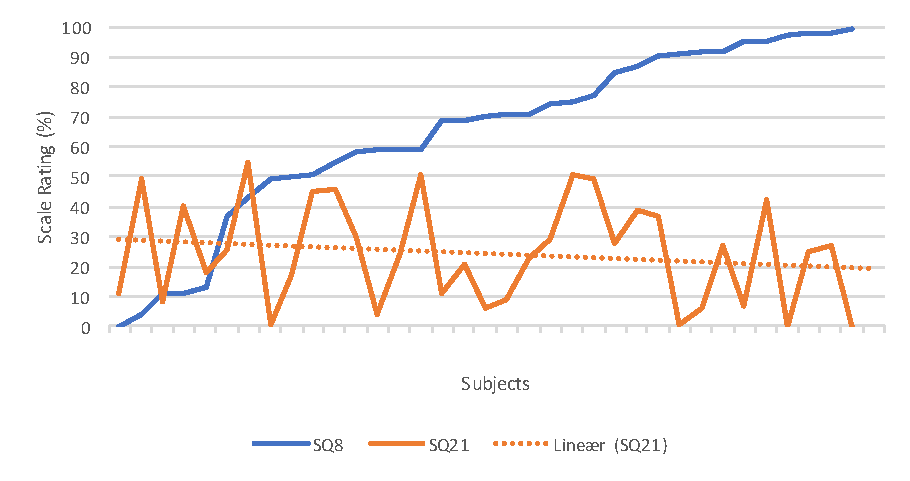
\includegraphics[width=\textwidth]{Figure/Korrelationsgrafer/SQ8+SQ21}
	\caption{Sammenhæng mellem hvad testpersonerne angiver (\%) på skalaen til SQ8: \textit{Jeg føler, at robotten kan hjælpe mig} og SQ21: \textit{Hvad synes du ellers om robotten?}. At den orange kurve ikke er kontinuerlig skyldes, at nogle testpersoner ikke har angivet en respons på skalaen.}
	\label{fig:SammenligningSQ8SQ21}
\end{figure}
\noindent
%
Undersøges den negative korrelation er sammenhængen mellem SQ2 og SQ9 allerede vist på \autoref{fig:SammenligningSQ2SQ9}. På \autoref{fig:SammenligningSQ14SQ16} vises sammenhængen for SQ14 og SQ16, hvor der ses en lille tendens for at robotten opleves som mindre sej, når den opleves som mere personlig. INGEN KORRELATION FORKERTE NÆVNTE PARAMETRE
%
\begin{figure}[H]
	\centering
	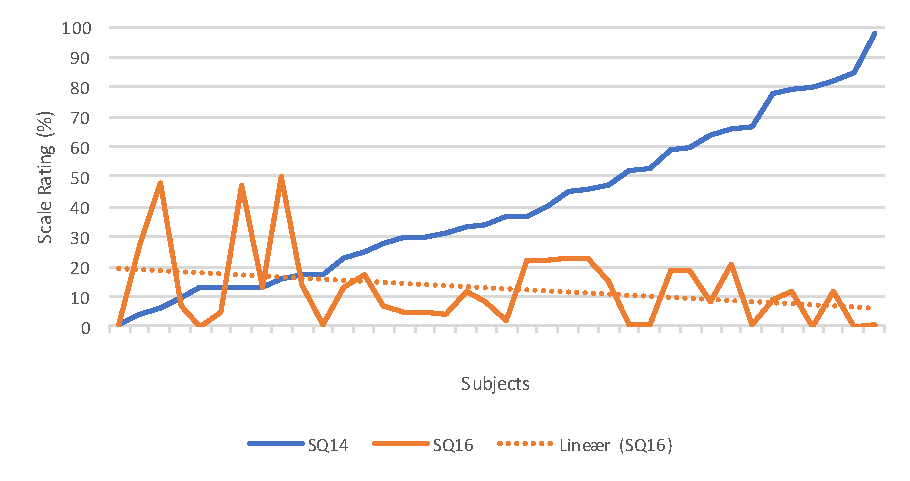
\includegraphics[width=\textwidth]{Figure/Korrelationsgrafer/SQ14+SQ16}
	\caption{Sammenhæng mellem hvad testpersonerne angiver (\%) på skalaen til SQ14: \textit{Hvor personlig oplevede du robottens hjælp?} og SQ16: \textit{Hvad synes du om robotten?}. At den orange kurve ikke er kontinuerlig skyldes, at nogle testpersoner ikke har angivet en respons på skalaen.}
	\label{fig:SammenligningSQ14SQ16}
\end{figure}
\noindent
%
Laves graferne for SQ10 og SQ13, SQ13 og SQ22 samt SQ19 og SQ20, vedlagt i \fullref{ELEKTRONISK BILAG}, ses det at graferne stiger samtidig. Dette er ikke forventet, da \autoref{fig:Distance-Biplot} viser en negativ korrelation ved disse parametre. Dog indikerer graferne at testpersonerne regnede med at blive fugt det sted de havde valgt, når de stolede på robotten og at robotten var sjov, når de troede de blev fulgt det rigtige sted hen. Ydermere indikerer graferne, at robotten blev perciperet som sej, når den også blev perciperet som sød.

Sammenlignes SQ5 og SQ8, jævnfør \autoref{fig:SammenligningSQ5SQ8}, er det svært at udlede, hvorvidt parametrene afhænger af hinanden eller følges ad ved tilfældighed. På trods af tidligere vist negativ korrelation relateret til afstand, virker det ikke til at testpersonerne har en ændret oplevelse af om robotten kan hjælpe dem, når robotten stopper tættere på eller længere væk. Det samme gør sig gældende, når SQ5 og SQ21 sammenlignes, hvilket kan ses på figuren i \fullref{ELEKTRONISK BILAG}. ORANGE STOR VARIATION OG BLÅ LILLE VARIATION  INGEN KORRELATION

\begin{figure}[H]
	\centering
	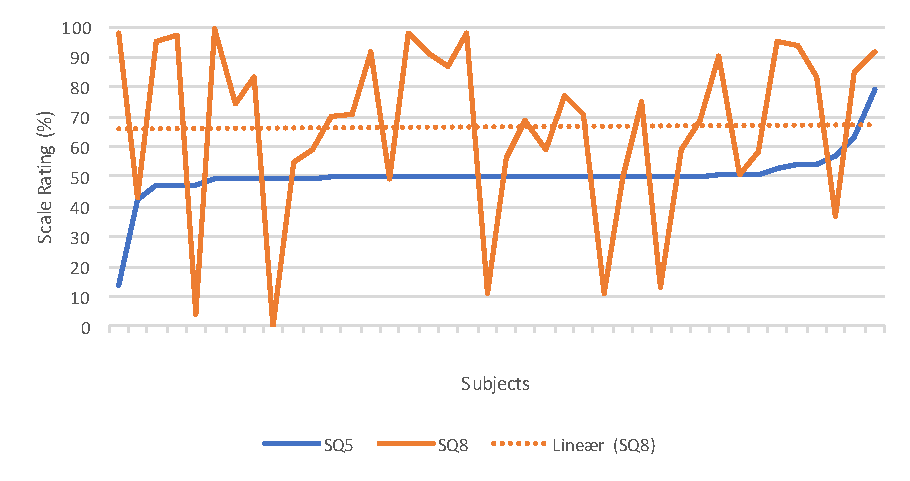
\includegraphics[width=\textwidth]{Figure/Korrelationsgrafer/SQ5+SQ8}
	\caption{Sammenhæng mellem hvad testpersonerne angiver (\%) på skalaen til SQ5: \textit{Jeg synes robotten stoppede...} og SQ8: \textit{Jeg føler, at robotten kan hjælpe mig}. At den orange kurve ikke er kontinuerlig skyldes, at nogle testpersoner ikke har angivet en respons på skalaen.}
	\label{fig:SammenligningSQ5SQ8}
\end{figure}

\subsubsection{Korrelation relativt til indgangsvinkel}
Når PCA analysen udføres relativt til indgangsvinkel, tyder det, som beskrevet i \fullref{DatabehandlingRIndgangsvinkel}, på, at en positiv korrelation mellem følgende parametre finder sted:
\begin{itemize}
	\item SQ8 og SQ10
	\item SQ9 og SQ14
	\item SQ5 og SQ7
\end{itemize}
%
Derudover ses der negativ korrelation mellem følgende parametre:
\begin{itemize}
	\item SQ1 og SQ12
	\item SQ9 og SQ10
	\item SQ10 og SQ14
	\item SQ6 og SQ23
	\item SQ13 og S21
\end{itemize}
%
Laves graferne for de positive korrelationer, SQ8 og SQ10, SQ9 og SQ14 samt SQ5 og SQ7 ses der ingen relevant sammenhæng, hvorfor disse kun medtages i det elektroniske bilag, \fullref{ELEKTRONISK BILAG}. Det samme gør sig gældende for de negative korrelationer, SQ1 og SQ12, SQ10 og SQ14 samt SQ6 og SQ23. 

Sammenlignes SQ9 og SQ10, jævnfør \autoref{fig:SammenligningSQ9SQ10} ses der en tendens, hvor testpersonerne føler sig mindre trygge ved robotten, jo mere de synes den stod i vejen. LILLE BITTE NEGATIV KORRELATION

%
\begin{figure}[H]
	\centering
	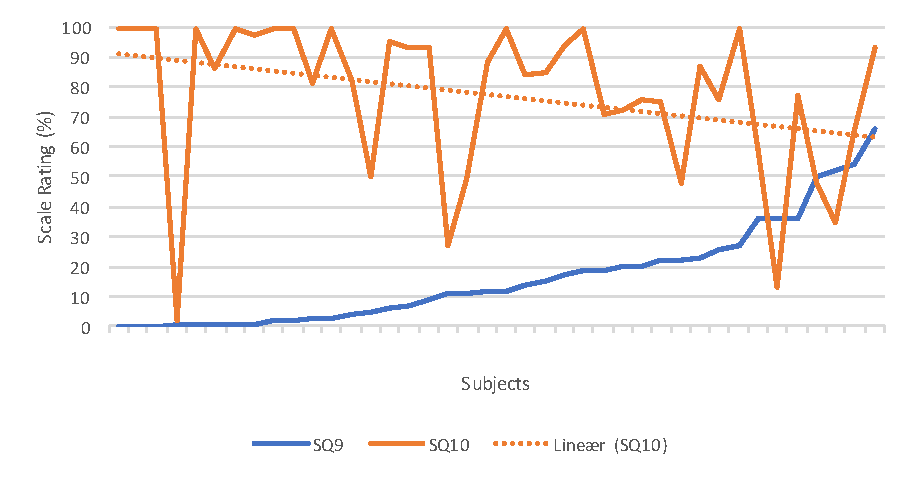
\includegraphics[width=\textwidth]{Figure/Korrelationsgrafer/SQ9+SQ10}
	\caption{Sammenhæng mellem hvad testpersonerne angiver (\%) på skalaen til SQ9: \textit{Jeg synes, at robotten stod i vejen} og SQ10: \textit{Jeg føler mig tryg ved robotten}.}
	\label{fig:SammenligningSQ9SQ10}
\end{figure}
\noindent
%
På \autopageref{fig:SammenligningSQ13SQ21} sammenlignes SQ13 og SQ21. Her ses en negativ korrelation mellem parametrene, hvor testpersonerne synes robotten blev mindre anmasende, når de regnede med den fulgte dem hen til det valgte sted. MÅSKR LILLE KORRELATION
%
\begin{figure}[H]
	\centering
	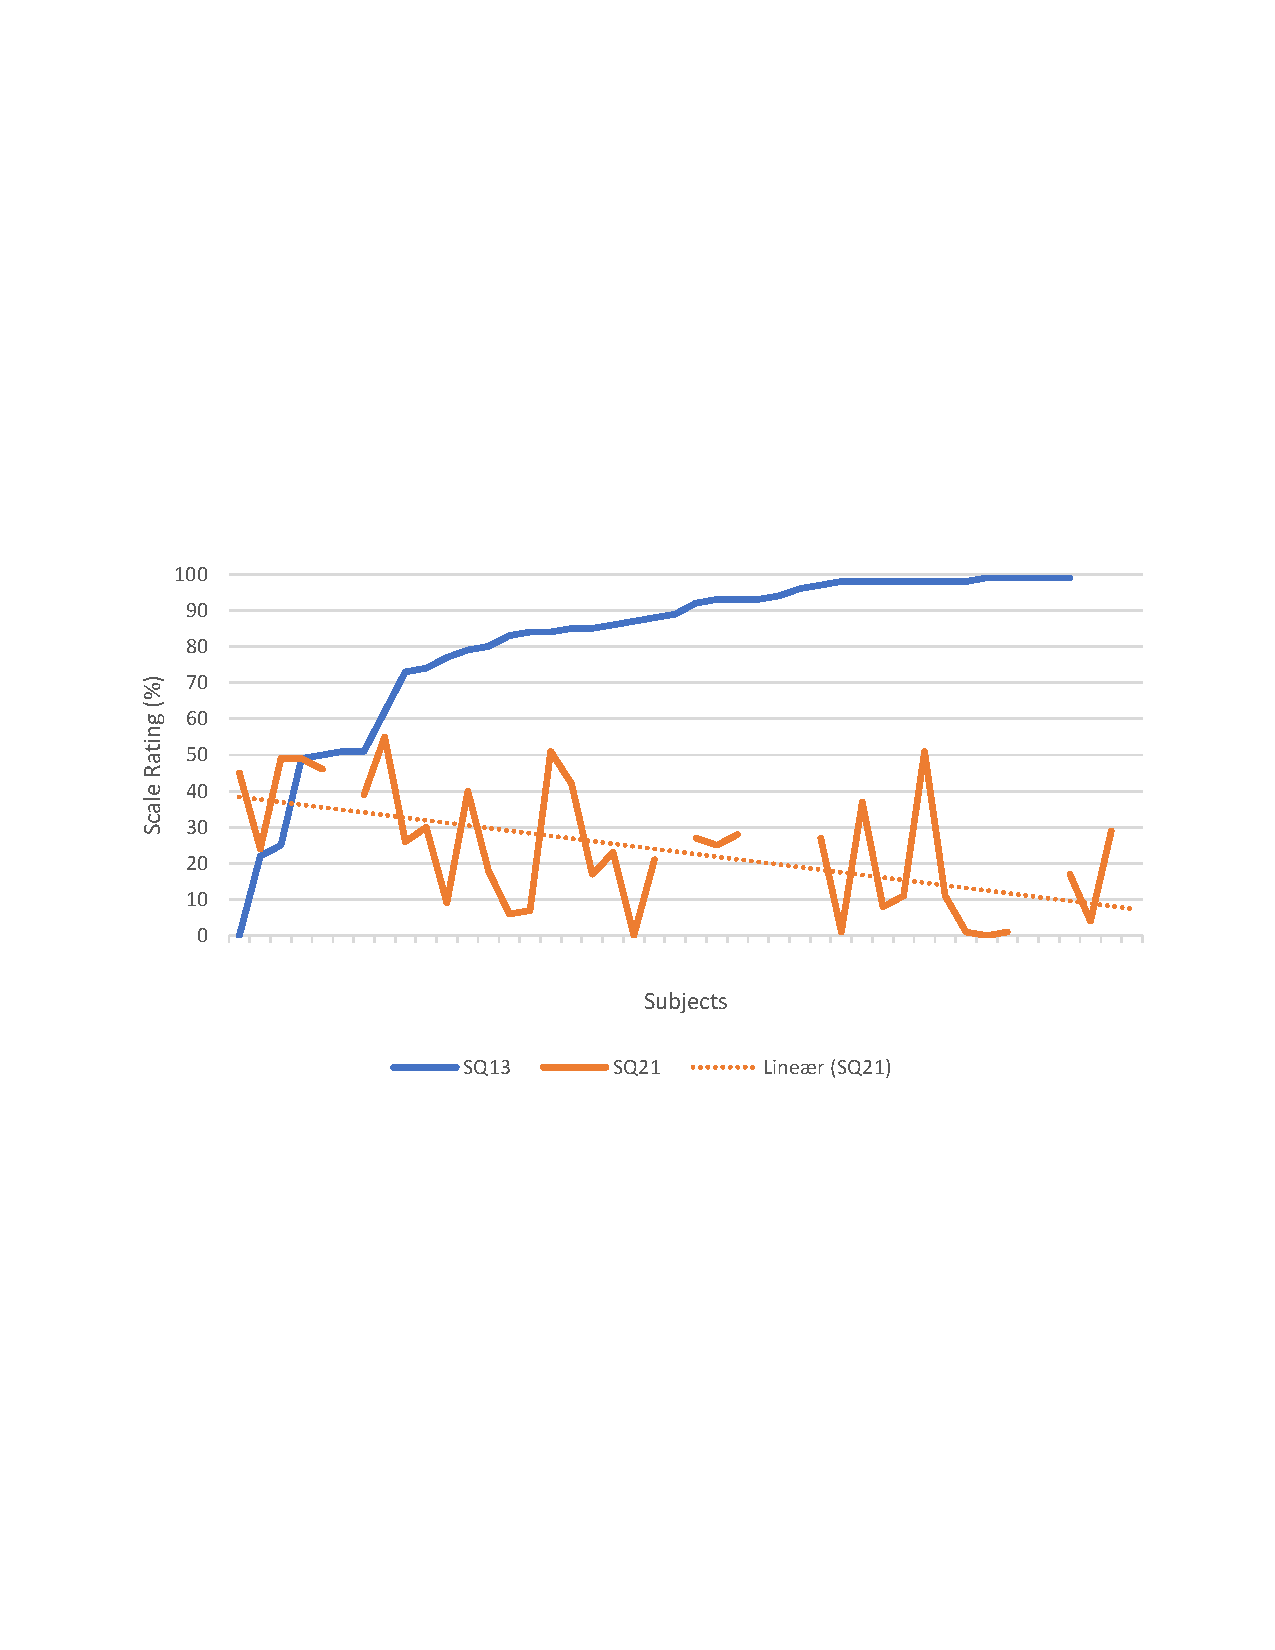
\includegraphics[width=\textwidth]{Figure/Korrelationsgrafer/SQ13+SQ21}
	\caption{Sammenhæng mellem hvad testpersonerne angiver (\%) på skalaen til SQ13: \textit{Jeg regnede med, at robotten fulgte mig hen til det sted jeg valgte} og SQ21: \textit{Hvad synes du ellers om robotten?}. At den orange kurve ikke er kontinuerlig skyldes, at nogle testpersoner ikke har angivet en respons på skalaen.}
	\label{fig:SammenligningSQ13SQ21}
\end{figure}
\noindent
%